Les \glspl{bdd} sont des outils permettant de stocker et retrouver des \glspl{data}, c'est à dire des valeurs brutes. 
Ces outils se trouvent au coeur des \glspl{si}, et sont indispensables aux entreprises.

En informatique, les bases de données sont numérisées, définies et manipulées grâce à des logiciels nommés \glspl{sgbd}.

Il existe différents types de bases de données, mais le marché reste dominé par les \glspl{bddr}\footnote{\label{part_de_marché_relationnel}
Classement des \glspl{sgbd} les plus populaires : \url{http://db-engines.com/en/ranking}}. Ces dernières sont gérées par des SGBD relationnels (dit SGBDR) 
dont les plus connus sont Oracle, MySQL et PostgreSQL.

Ces logiciels permettent de définir et de manipuler des bases de données par le biais du \gls{sql}, 
langage déclaratif et normé qui reste le premier et le plus exhaustif des moyens de gérer une base de données relationnelle .

Mais le SQL est un langage informatique, ce qui constitue un frein pour les utilisateurs : s'ils ne connaissent pas
le langage, ils ne peuvent pas utiliser de base de données.

Certaines applications, comme \textit{Access}, \textit{LOBase} ou encore \textit{phpMyAdmin} proposent une alternative au SQL grâce à des 
\glspl{ihm}: il est possible de définir les données ou de les manipuler par des clics de boutons, des glisser-déplacer, des cases à cocher ou encore de la saisie
de texte non codé. 

En suivant cette optique, le but de ce projet tuteuré est de réaliser une application permettant d'utiliser certaines fonctionnalités 
des bases de données \underline{sans} 
avoir recours au SQL, et ce sur n'importe quel SGBDR. Pour cela, elle propose une série d'IHM qui en reprennent certaines fonctionnalités,
à savoir le \gls{ldd} et le \gls{lmd}.

Les utilisateurs finaux de l'application sont les élèves de première année du DUT Informatique, pour
les aider à découvrir les bases de données.

Ce document présente les différentes phases de création de cette application : l'analyse, la conception, le développement et les tests.
Un manuel d'utilisation est disponible dans les dernières pages.

Afin de mieux situer l'application, la figure \ref{sans_idb_schema} montre l'utilisation classique d'un SGBD et 
la figure \ref{avec_idb_schema} l'utilisation de l'application développée.

\begin{figure}[!h]
  \centering
  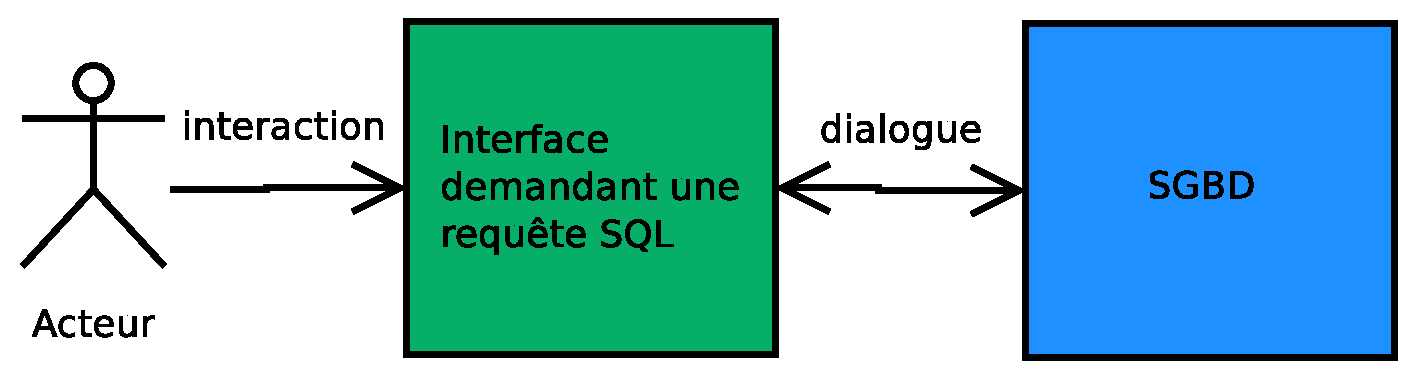
\includegraphics[width=14cm]{images/sans_idb.eps}
  \caption{Utilisation classique d'un SGBD.}
  \label{sans_idb_schema}
\end{figure}

\begin{figure}[!h]
  \centering
  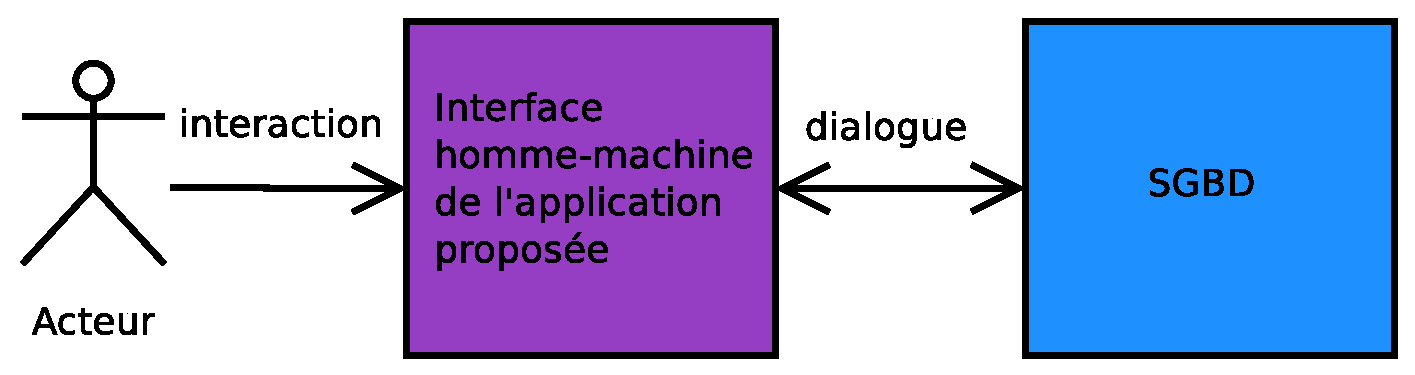
\includegraphics[width=14cm]{images/avec_idb.eps}
  \caption{Utilisation d'un SGBD avec l'application du projet.}
  \label{avec_idb_schema}
\end{figure}
%TODO : donner un nom à l'application
